\chapter{Clustering}


% ---------- Mutual Info Score ----------
\clearpage
\thispagestyle{clusteringstyle}
\section{Mutual Info Score}
\subsection{Mutual Info Score}

% ---------- adjusted mutual info score ----------
\clearpage
\thispagestyle{clusteringstyle}
\section{Adjusted Mutual Info score}
\subsection{Adjusted Mutual Information score}

% ---------- Normalized Mutual Info Score ----------
\clearpage
\thispagestyle{clusteringstyle}
\section{Normalized Mutual Info Score}
\subsection{Normalized Mutual Info Score}

% ---------- rand score ----------
\clearpage
\thispagestyle{clusteringstyle}
\section{Rand Score}
\subsection{Rand Score}

% ---------- adjusted rand score ----------
\clearpage
\thispagestyle{clusteringstyle}
\section{Adjusted Rand Score}
\subsection{Adjusted Rand Score}

% ---------- calinski harabasz score ----------
\clearpage
\thispagestyle{clusteringstyle}
\section{CH Score}
\subsection{Calinski Harabasz Score}


% ---------- contingency matrix ----------
\clearpage
\thispagestyle{clusteringstyle}
\section{Contingency Matrix}
\subsection{Contingency Matrix}

% ---------- pair confusion matrix ----------
\clearpage
\thispagestyle{clusteringstyle}
\section{Pair Confusion Matrix}
\subsection{Pair Confusion Matrix}

% ---------- Completeness Score ----------
\clearpage
\thispagestyle{clusteringstyle}
\section{Completeness Score}
\subsection{Completeness Score}

% ---------- Davis Bouldin Score ----------
\clearpage
\thispagestyle{clusteringstyle}
\section{Davis Bouldin Score}
\subsection{Davis Bouldin Score}

% ---------- Fowlkes Mallows Score ----------
\clearpage
\thispagestyle{clusteringstyle}
\section{Fowlkes Mallows Score}
\subsection{Fowlkes Mallows Score}

% ---------- Homogeneity Score ----------
\clearpage
\thispagestyle{clusteringstyle}
\section{Homogeneity Score}
\subsection{Homogeneity Score}

% ---------- V Measure ----------
\clearpage
\thispagestyle{clusteringstyle}
\section{V Measure}
\subsection{V Measure}

% ---------- Homogeneity Completeness V Measure ----------
\clearpage
\thispagestyle{clusteringstyle}
\section{Homogeneity Completeness V Measure}
\subsection{Homogeneity Completeness V Measure}

% ---------- Silhouette Score ----------
\clearpage
\thispagestyle{clusteringstyle}
\section{Silhouette Score}
\subsection{Silhouette Score}

The Silhouette Coefficient measures how well a data point fits within its assigned cluster compared to other clusters. 
It quantifies how similar a sample is to its own cluster (cohesion) compared to the nearest neighboring cluster (separation).
The Silhouette Coefficient $s(i)$ for a given data point $i$ in the cluster $C_I$, where $|C_I|$ is the number of data points in $C_I$, is given by:

\begin{center}
\tikz{
\node[inner sep=2pt, font=\Large] (a) {
{
$\displaystyle
s(i) = 
\begin{cases}
\frac{{\color{cyan}b(i)} - {\color{nmlpurple}a(i)}}{max\left\{ {\color{nmlpurple}a(i)}, {\color{cyan}b(i)} \right\}}  & if\, |C_I| > 1 \\
0  & if\, |C_I| = 1
\end{cases}
$
}
};
\draw[-latex,cyan, semithick] ($(a.north)+(-0.9,0.05)$) to[bend right=15] node[pos=1, left] {measures cohesion} +(-1,.5); 
\draw[-latex,nmlpurple, semithick] ($(a.north)+(0.2,0.05)$) to[bend left=15] node[pos=1, right] {measures separation} +(1,.5); 
% \draw[-latex,nmlpurple, semithick] ($(b.north)+(0.1,0.05)$) to[bend left=15] node[pos=1, left] {True negatives} +(-1,-.5); 
}
\end{center}

Where  $a(i)$ is the mean distance between a sample and all other points in the same cluster (mean intra-cluster distance), 
and  $b(i)$ is the mean distance between a sample and all points in the nearest different cluster (mean nearest-cluster distance). 
The value of  $s(i)$ lies between -$1$ and  $1$, where  $s(i) \approx 1$ indicates that the data point is well-clustered, 
 $s(i) \approx 0$ means the data point is on or very close to the boundary between two clusters, and  $s(i) \approx -1$ 
suggests that the data point has been misclassified into the wrong cluster.

\textbf{When to use Silhouette Score?}

Use Silhouette Score when the ground truth labels are unknown and the evaluation must be performed using the model itself.

\coloredboxes{
\item It provides a clear and intuitive measure of how well clusters are separated, +1 highly dense and -1 for incorrect clustering.
}
{
\item Silhouette Score can generally be higher for convex clusters than other clusters, such as density based clusters.
\item Higher Silhouette Score doesn't necessarily indicate that the clusters will have equal sizes; the clusters can still vary in cardinality. 
}

% ----------  Consensus Score ----------
\clearpage
\thispagestyle{clusteringstyle}
\section{ Consensus Score}
\subsection{ Consensus Score}


% ----------  Dunn Index ----------
\clearpage
\thispagestyle{clusteringstyle}
\section{ Dunn Index}

% Define colors
\definecolor{nmlpurple}{RGB}{128,0,128}

The Dunn Index is used to evaluate the quality of clusters by measuring both the separation between the clusters and compactness within clusters. It considers the smallest distance between points in different clusters (inter-cluster distance) and the largest distance within a single cluster (intra-cluster distance) to evaluate how well-defined the clusters are. A higher Dunn Index indicates that the clustering configuration has well-separated and compact clusters, while a lower Dunn Index suggests poor separation or high dispersion within clusters.\\

The Dunn Index for a given clustering solution with \( k \) clusters \( C_1, C_2, \ldots, C_k \) is defined as:

\begin{center}
	\begin{tikzpicture}
		\node[inner sep=2pt, font=\Large] (a) {
			$\displaystyle
			D = \frac{\min\limits_{1 \leq i < j \leq k} \{ \text{dist}(C_i, C_j) \}}{\max\limits_{1 \leq i \leq k} \{ \text{diam}(C_i) \}}
			$
		};
		\draw[-latex, cyan, semithick] ($(a.north east)+(0.2,-0.1)$) to[bend left=15] node[pos=1, right] {measures inter-cluster distance} +(2,0.5); 
		\draw[-latex, nmlpurple, semithick] ($(a.south east)+(0.2,0.1)$) to[bend right=15] node[pos=1, right] {measures intra-cluster distance} +(2,-0.5); 
	\end{tikzpicture}
\end{center}

where:
\begin{itemize}
	\item \(\text{dist}(C_i, C_j)\) represents the distance between clusters \( C_i \) and \( C_j \), often calculated as the minimum distance between any two points in different clusters (inter-cluster distance).
	\item \(\text{diam}(C_i)\) represents the diameter of cluster \( C_i \), typically defined as the maximum distance between any two points within the same cluster (intra-cluster distance).
\end{itemize}

\textit{The Dunn Index ranges from 0 to infinity, with higher values indicating better-defined clusters. Values closer to 0 suggest that clusters are either overlapping or not sufficiently compact.}\\

\textbf{When to Use Dunn Index?}

The Dunn Index is primarily used when evaluating clustering results in applications where the structure and separation of clusters are critical. It is useful in determining whether a clustering algorithm has successfully created distinct, dense clusters without overlap. The Dunn Index is particularly valuable for comparing clustering algorithms, such as K-means, hierarchical clustering, and DBSCAN, especially when the number of clusters is uncertain, or various configurations need to be tested.

% strength and weakness box
\coloredboxes{
	\item Considers both intra-cluster compactness and inter-cluster separation.
	\item Useful for determining the best number of clusters.
	\item Higher values indicate better-defined clusters.
	\item Helps compare clustering algorithms.
}
{
	\item Outliers can reduce the Dunn Index value, affecting accuracy.
	\item High resource use for large datasets.
	\item Less effective for irregular shapes.
	\item Sensitive to unnormalized features.
	\item Can be unreliable in high-dimensional spaces.
}

% Inserting the image
\begin{figure}[h!]
	\centering
	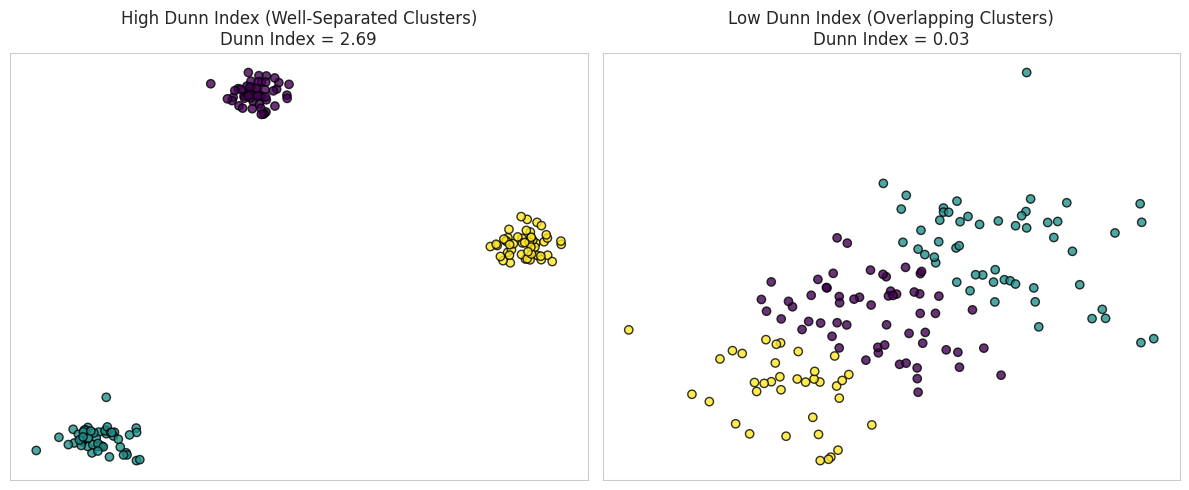
\includegraphics[width=\textwidth]{/figures/Dunn_Index_Visualized.png} 
	\caption{Illustration of High and Low Dunn Index Values}
\end{figure}

% Adding the explanation below the image
\textbf{In the visualization above:}
\begin{itemize}
	\item \textbf{Left Plot (High Dunn Index):} This example illustrates clusters that are well-separated and compact. Each cluster (shown in blue, green, and purple) is distinct, with clear boundaries and minimal overlap with other clusters. The points within each cluster are closely packed, which leads to a small maximum intra-cluster distance (diameter). Furthermore, the minimum distance between clusters (inter-cluster distance) is large, reinforcing the separation between clusters. These characteristics yield a high Dunn Index, signifying a high-quality clustering configuration where clusters are well-defined and do not overlap.
	\item \textbf{Right Plot (Low Dunn Index):} This example illustrates clusters that are overlapping and dispersed. The clusters lack distinct boundaries, and points from different clusters are intermixed. The large maximum intra-cluster distance, due to dispersed points within clusters, combined with a small minimum inter-cluster distance, because of overlapping clusters, results in a low Dunn Index. This clustering configuration suggests poor clustering quality, as the clusters are not compact or well-separated.
\end{itemize}

\subsection{ Dunn Index}

